\documentclass{beamer}\usepackage[]{graphicx}\usepackage[]{color}
%% maxwidth is the original width if it is less than linewidth
%% otherwise use linewidth (to make sure the graphics do not exceed the margin)
\makeatletter
\def\maxwidth{ %
  \ifdim\Gin@nat@width>\linewidth
    \linewidth
  \else
    \Gin@nat@width
  \fi
}
\makeatother

\definecolor{fgcolor}{rgb}{0.345, 0.345, 0.345}
\newcommand{\hlnum}[1]{\textcolor[rgb]{0.686,0.059,0.569}{#1}}%
\newcommand{\hlstr}[1]{\textcolor[rgb]{0.192,0.494,0.8}{#1}}%
\newcommand{\hlcom}[1]{\textcolor[rgb]{0.678,0.584,0.686}{\textit{#1}}}%
\newcommand{\hlopt}[1]{\textcolor[rgb]{0,0,0}{#1}}%
\newcommand{\hlstd}[1]{\textcolor[rgb]{0.345,0.345,0.345}{#1}}%
\newcommand{\hlkwa}[1]{\textcolor[rgb]{0.161,0.373,0.58}{\textbf{#1}}}%
\newcommand{\hlkwb}[1]{\textcolor[rgb]{0.69,0.353,0.396}{#1}}%
\newcommand{\hlkwc}[1]{\textcolor[rgb]{0.333,0.667,0.333}{#1}}%
\newcommand{\hlkwd}[1]{\textcolor[rgb]{0.737,0.353,0.396}{\textbf{#1}}}%
\let\hlipl\hlkwb

\usepackage{framed}
\makeatletter
\newenvironment{kframe}{%
 \def\at@end@of@kframe{}%
 \ifinner\ifhmode%
  \def\at@end@of@kframe{\end{minipage}}%
  \begin{minipage}{\columnwidth}%
 \fi\fi%
 \def\FrameCommand##1{\hskip\@totalleftmargin \hskip-\fboxsep
 \colorbox{shadecolor}{##1}\hskip-\fboxsep
     % There is no \\@totalrightmargin, so:
     \hskip-\linewidth \hskip-\@totalleftmargin \hskip\columnwidth}%
 \MakeFramed {\advance\hsize-\width
   \@totalleftmargin\z@ \linewidth\hsize
   \@setminipage}}%
 {\par\unskip\endMakeFramed%
 \at@end@of@kframe}
\makeatother

\definecolor{shadecolor}{rgb}{.97, .97, .97}
\definecolor{messagecolor}{rgb}{0, 0, 0}
\definecolor{warningcolor}{rgb}{1, 0, 1}
\definecolor{errorcolor}{rgb}{1, 0, 0}
\newenvironment{knitrout}{}{} % an empty environment to be redefined in TeX

\usepackage{alltt}
\usepackage{amsfonts} % Worcester's
\usepackage{amssymb, amsfonts, latexsym, amsmath}
\usepackage{multirow,array,graphicx,rotating,epsfig}
\usepackage{verbatim}
\usepackage{enumerate}
\usepackage{color}
\usepackage{multicol}
\usepackage{subfig}
\usepackage{float}
\usepackage{setspace}
\renewenvironment{knitrout}{\begin{singlespace}}{\end{singlespace}}
%\usepackage{hyperref}

\hypersetup{
colorlinks=true,
urlcolor=cyan,
linkcolor=blue  
}

\newcommand{\ba}{{\bf a}}
\newcommand{\bA}{{\bf A}}
\newcommand{\mcA}{{\mathcal A}}
\newcommand{\bB}{{\bf B}}
\newcommand{\bb}{{\bf b}}
\newcommand{\mfB}{{\mathfrak B}}
\newcommand{\mcB}{{\mathcal B}}
\newcommand{\bc}{{\bf c}}
\newcommand{\bC}{{\bf C}}
\newcommand{\mcC}{{\mathcal C}}
\newcommand{\mbC}{{\mathbb C}}
\newcommand{\mcD}{{\mathcal D}}
\newcommand{\be}{{\bf e}}
\newcommand{\bE}{{\bf E}}
\newcommand{\mcF}{{\mathcal F}}
\newcommand{\mcG}{{\mathcal G}}
\newcommand{\bh}{{\bf h}}
\newcommand{\bH}{{\bf H}}
\newcommand{\mcH}{{\mathcal H}}
\newcommand{\mbH}{{\mathbb H}}
\newcommand{\mcI}{{\mathcal I}}
\newcommand{\bK}{{\bf K}}
\newcommand{\mcL}{{\mathcal L}}
\newcommand{\mcN}{{\mathcal N}}
\newcommand{\mcP}{{\mathcal P}}
\newcommand{\bq}{{\bf q}}
\newcommand{\bQ}{{\bf Q}}
\newcommand{\mbR}{{\mathbb R}}
\newcommand{\bR}{{\bf R}}
\newcommand{\mcS}{{\mathcal S}}
\newcommand{\mfS}{{\mathfrak S}}
\newcommand{\bs}{{\bf s}}
\newcommand{\mcT}{{\mathcal T}}
\newcommand{\bv}{{\bf v}}
\newcommand{\bV}{{\bf V}}
\newcommand{\mcV}{{\mathcal V}}
\newcommand{\bW}{{\bf W}}
\newcommand{\bw}{{\bf w}}
\newcommand{\bX}{{\bf X}}
\newcommand{\bx}{{\bf x}}
\newcommand{\bY}{{\bf Y}}
\newcommand{\bZ}{{\bf Z}}

\newcommand{\bzero}{{\bf 0}}
\newcommand{\bone}{{\bf 1}}

\newcommand{\bbeta}{{\boldsymbol{\beta}}}
\newcommand{\bep}{{\boldsymbol{\vep}}}
\newcommand{\bmu}{{\boldsymbol{\mu}}}
\newcommand{\vep}{\varepsilon}
\newcommand{\bvep}{{\boldsymbol{\vep}}}
%\newcommand{\bVep}{{\boldsymbol{\Varepsilon}}}
\newcommand{\bLambda}{{\boldsymbol{\Lambda}}}
\newcommand{\bPhi}{{\boldsymbol{\varPhi}}}
\newcommand{\bSigma}{{\boldsymbol{\Sigma}}}
\newcommand{\bxi}{{\boldsymbol{\xi}}}
\newcommand{\bXi}{{\boldsymbol{\Xi}}}

\DeclareMathOperator\E{E}
\DeclareMathOperator\Cov{Cov}
\DeclareMathOperator\Corr{Corr}
\DeclareMathOperator\diag{diag}
\DeclareMathOperator\logit{logit}
\DeclareMathOperator\sign{sign}
\DeclareMathOperator\Span{span}
\DeclareMathOperator\vc{vec}
\DeclareMathOperator\Var{Var}
\DeclareMathOperator\trace{trace}

\DeclareMathOperator\convD{\overset{\mcD}{\to}}
\DeclareMathOperator\convP{\overset{\mcP}{\to}}
\DeclareMathOperator\convas{\overset{as}{\to}}



%%%%%% Beamer Options
%\useoutertheme{infolines}
\definecolor{PSUblue}{RGB}{0,48,135}
\beamertemplatenavigationsymbolsempty
\setbeamerfont{page number in head/foot}{size=\small}
\setbeamertemplate{footline}[frame number]
%\addtobeamertemplate{headline}{}{\rule{\paperwidth}{3pt}}
\makeatletter
\def\th@mystyle{%
    \normalfont % body font
    \setbeamercolor{block title example}{bg=PSUblue,fg=white}
    \setbeamercolor{block body example}{bg=PSUblue!20,fg=black}
    \def\inserttheoremblockenv{exampleblock}
}
\makeatother
\theoremstyle{mystyle}
\newtheorem{mytheorem}{Theorem}


%%%%%% Knitr Options
\usepackage{etoolbox} 
\makeatletter 
\preto{\@verbatim}{\topsep=0pt \partopsep=0pt } 
\makeatother
\IfFileExists{upquote.sty}{\usepackage{upquote}}{}
\begin{document}
% \SweaveOpts{concordance=TRUE}
% <<echo=FALSE,results='hide',message=FALSE>>=
% opts_knit$set(width=20,out.width=20)
% options(width=50)
% library(fda)
% library(refund)
% set.seed(2016)
% @

\title{
Data Types, Vectors, and Subsetting
}
\author{
}
\date{}

\begin{frame}[fragile]
\titlepage
\end{frame}


\begin{frame}{Data analyst's perspective}
\begin{itemize}
\item Think in terms of variables – an ordered collection of measurements on a group of subjects
\item Care about the kind of measuremet values: it informs the type of analysis we might perform, e.g., it makes sense to compute the mean/median of numeric values, but not categorical values
\item Care about missing data – we adjust our analyses depending on the amount and kind of missingness
\end{itemize}
\end{frame}

\begin{frame}[fragile]{Data types}
\begin{itemize}
\item R has a number of built-in data types.  The three most basic types are numeric, character, and logical 
\item You can check the type using the class function.
\end{itemize}
\begin{singlespace}
\begin{knitrout}
\definecolor{shadecolor}{rgb}{0.969, 0.969, 0.969}\color{fgcolor}\begin{kframe}
\begin{alltt}
\hlkwd{class}\hlstd{(}\hlnum{3.5}\hlstd{)}
\end{alltt}
\begin{verbatim}
## [1] "numeric"
\end{verbatim}
\begin{alltt}
\hlkwd{class}\hlstd{(}\hlstr{"Hello there"}\hlstd{)}
\end{alltt}
\begin{verbatim}
## [1] "character"
\end{verbatim}
\begin{alltt}
\hlkwd{class}\hlstd{(}\hlnum{TRUE}\hlstd{)}
\end{alltt}
\begin{verbatim}
## [1] "logical"
\end{verbatim}
\end{kframe}
\end{knitrout}
\end{singlespace}
\begin{itemize}
\item Another important type is factor
\end{itemize}
\end{frame}


\begin{frame}{Note about data types}
\begin{itemize}
\item Actually, the types are numeric, character, and logical vectors.  There’s no such thing as a scalar in R, just a vector of length one.
\end{itemize}
\end{frame}

\begin{frame}[fragile]{Vectors}
\begin{center}
    {{\resizebox*{1.1\textwidth}{1.1\textheight}
        {\rotatebox{0}{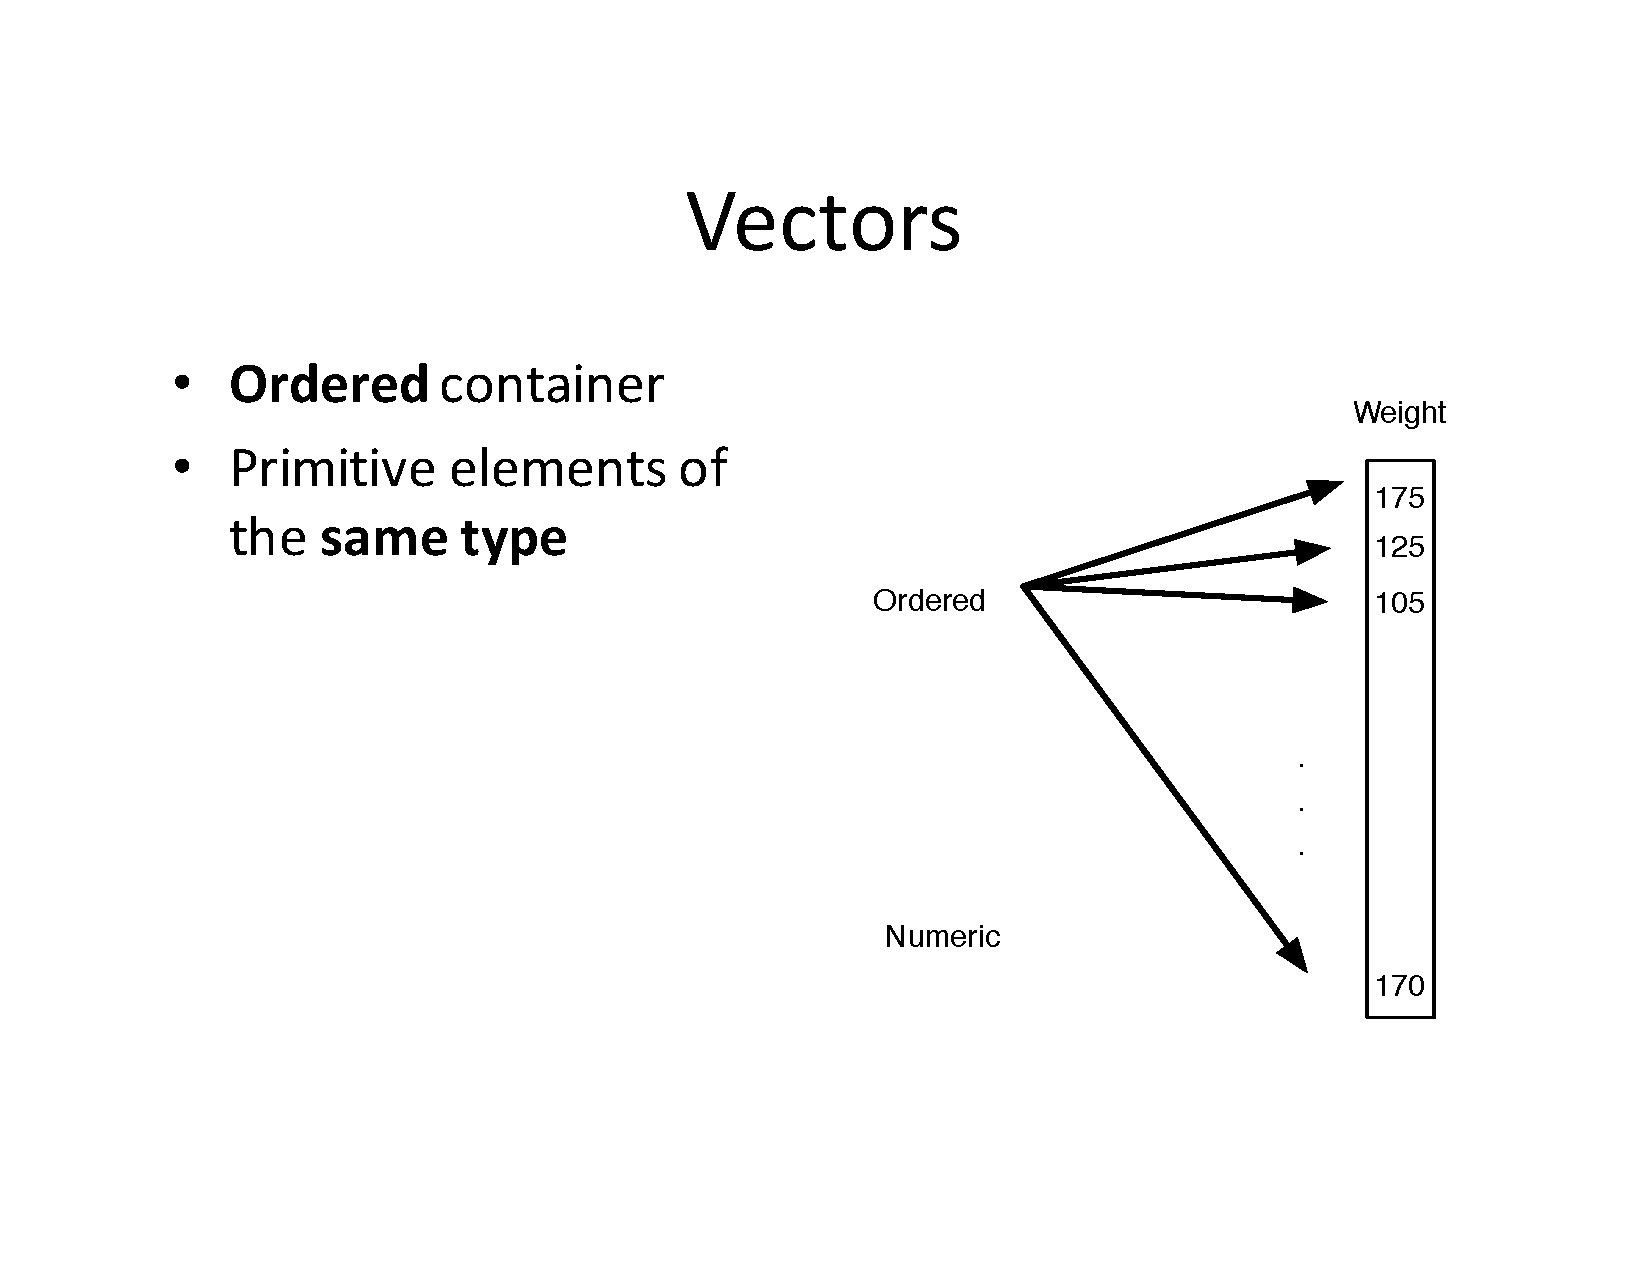
\includegraphics{Vectors.pdf}}}} \par}
  \end{center}
\end{frame}

\begin{frame}[fragile]{Vectors: family data example}
\begin{itemize}
\item We have data on a 14-member family – vectors of first names, age, gender, weight, height, whether or not they are over weight (BMI above 25).
\item What are the data types?
\begin{knitrout}
\definecolor{shadecolor}{rgb}{0.969, 0.969, 0.969}\color{fgcolor}\begin{kframe}
\begin{alltt}
\hlkwd{load}\hlstd{(}\hlkwd{url}\hlstd{(}
  \hlstr{"http://www.stat.berkeley.edu/users/nolan/data/afamily.rda"}\hlstd{))}
\end{alltt}
\end{kframe}
\end{knitrout}
\item More readable:\\ load(url(
"http://www.stat.berkeley.edu/
users/nolan/data/afamily.rda"))
\end{itemize}
\end{frame}

\begin{frame}[fragile]{First names and ages}
\begin{knitrout}
\definecolor{shadecolor}{rgb}{0.969, 0.969, 0.969}\color{fgcolor}\begin{kframe}
\begin{alltt}
\hlstd{fnames}
\end{alltt}
\begin{verbatim}
##  [1] "Tom"    "Maya"   "Joe"    "Robert" "Sue"    "Liz"    "Jon"   
##  [8] "Sally"  "Tim"    "Tom"    "Ann"    "Dan"    "Art"    "Zoe"
\end{verbatim}
\begin{alltt}
\hlkwd{class}\hlstd{(fnames)}
\end{alltt}
\begin{verbatim}
## [1] "character"
\end{verbatim}
\begin{alltt}
\hlstd{fage}
\end{alltt}
\begin{verbatim}
##  [1] 77 33 79 47 27 33 67 52 59 27 55 24 46 48
\end{verbatim}
\begin{alltt}
\hlkwd{class}\hlstd{(fage)}
\end{alltt}
\begin{verbatim}
## [1] "integer"
\end{verbatim}
\end{kframe}
\end{knitrout}
\end{frame}

\begin{frame}[fragile]{Gender and over weight}
\begin{knitrout}
\definecolor{shadecolor}{rgb}{0.969, 0.969, 0.969}\color{fgcolor}\begin{kframe}
\begin{alltt}
\hlstd{fsex}
\end{alltt}
\begin{verbatim}
##  [1] m f m m f f m f m m f m m f
## Levels: f m
\end{verbatim}
\begin{alltt}
\hlkwd{class}\hlstd{(fsex)}
\end{alltt}
\begin{verbatim}
## [1] "factor"
\end{verbatim}
\begin{alltt}
\hlstd{foverWt}
\end{alltt}
\begin{verbatim}
##  [1]  TRUE FALSE FALSE FALSE FALSE  TRUE  TRUE FALSE  TRUE  TRUE  TRUE
## [12] FALSE FALSE FALSE
\end{verbatim}
\begin{alltt}
\hlkwd{class}\hlstd{(foverWt)}
\end{alltt}
\begin{verbatim}
## [1] "logical"
\end{verbatim}
\end{kframe}
\end{knitrout}
\end{frame}

\begin{frame}[fragile]{More on data types}
\begin{itemize}
\item A logical vector contains values that are either TRUE or FALSE. 
\item A factor vector is a special storage class used for qualitative data. The values are internally stored as integers by each integer corresponds to a level, which is a character string
\end{itemize}
\begin{knitrout}
\definecolor{shadecolor}{rgb}{0.969, 0.969, 0.969}\color{fgcolor}\begin{kframe}
\begin{alltt}
\hlkwd{levels}\hlstd{(fsex)}
\end{alltt}
\begin{verbatim}
## [1] "f" "m"
\end{verbatim}
\end{kframe}
\end{knitrout}
\end{frame}

\begin{frame}[fragile]{Special values}
\begin{itemize}
\item The missing value symbol is NA  
\item It stands for “Not Available”
\item NA can be an element of a vector of any type  
\item NA is different from the character string “NA” 
\item You can check for the presence of NA values using the is.na() function.
\end{itemize}
\end{frame}

\begin{frame}[fragile]{Special values}
\begin{itemize}
\item Other special values are NaN, for “not a number,” which typically arises when you try to compute an indeterminate form such as 0/0.
\begin{knitrout}
\definecolor{shadecolor}{rgb}{0.969, 0.969, 0.969}\color{fgcolor}\begin{kframe}
\begin{alltt}
\hlnum{0}\hlopt{/}\hlnum{0}
\end{alltt}
\begin{verbatim}
## [1] NaN
\end{verbatim}
\end{kframe}
\end{knitrout}
\item The result of dividing a non-zero number by zero is Inf (or -Inf).
\begin{knitrout}
\definecolor{shadecolor}{rgb}{0.969, 0.969, 0.969}\color{fgcolor}\begin{kframe}
\begin{alltt}
\hlnum{12}\hlopt{/}\hlnum{0}
\end{alltt}
\begin{verbatim}
## [1] Inf
\end{verbatim}
\end{kframe}
\end{knitrout}
\end{itemize}
\end{frame}

\begin{frame}[fragile]{Special values}
\begin{itemize}
\item Other special values are NaN, for “not a number,” which typically arises when you try to compute an indeterminate form such as 0/0.
\begin{knitrout}
\definecolor{shadecolor}{rgb}{0.969, 0.969, 0.969}\color{fgcolor}\begin{kframe}
\begin{alltt}
\hlnum{0}\hlopt{/}\hlnum{0}
\end{alltt}
\begin{verbatim}
## [1] NaN
\end{verbatim}
\end{kframe}
\end{knitrout}
\item The result of dividing a non-zero number by zero is Inf (or -Inf).
\begin{knitrout}
\definecolor{shadecolor}{rgb}{0.969, 0.969, 0.969}\color{fgcolor}\begin{kframe}
\begin{alltt}
\hlnum{12}\hlopt{/}\hlnum{0}
\end{alltt}
\begin{verbatim}
## [1] Inf
\end{verbatim}
\end{kframe}
\end{knitrout}
\end{itemize}
\end{frame}

\begin{frame}[fragile]{Special values}
\begin{itemize}
\item NULL is a special value value that denotes an empty vector
\begin{knitrout}
\definecolor{shadecolor}{rgb}{0.969, 0.969, 0.969}\color{fgcolor}\begin{kframe}
\begin{alltt}
\hlkwd{names}\hlstd{(fweight)}
\end{alltt}
\begin{verbatim}
## NULL
\end{verbatim}
\end{kframe}
\end{knitrout}
\item Here we asked for the names of the elements of the vector fweight. The function names returns a character vector of element names. Since this vector has no element names, the return value is a NULL vector
\end{itemize}
\end{frame}

\begin{frame}[fragile]{Finding out more information}
\begin{itemize}
\item Retrieve the number of elements in the vector
\item Examine the first 6 elements in the vector
\item Elements can have names – height has names 
\item Are any of the elements in the vector missing?
\end{itemize}
\end{frame}

\begin{frame}[fragile]{Finding out information: R code}
\begin{knitrout}
\definecolor{shadecolor}{rgb}{0.969, 0.969, 0.969}\color{fgcolor}\begin{kframe}
\begin{alltt}
\hlkwd{length}\hlstd{(fweight)}
\end{alltt}
\begin{verbatim}
## [1] 14
\end{verbatim}
\begin{alltt}
\hlkwd{head}\hlstd{(fweight)}
\end{alltt}
\begin{verbatim}
## [1] 175 124 185 156  98 190
\end{verbatim}
\begin{alltt}
\hlkwd{names}\hlstd{(fheight)}
\end{alltt}
\begin{verbatim}
##  [1] "a" "b" "c" "d" "e" "f" "g" "h" "i" "j" "k" "l" "m" "n"
\end{verbatim}
\begin{alltt}
\hlkwd{is.na}\hlstd{(fweight)}
\end{alltt}
\begin{verbatim}
##  [1] FALSE FALSE FALSE FALSE FALSE FALSE FALSE FALSE FALSE FALSE FALSE
## [12] FALSE FALSE FALSE
\end{verbatim}
\end{kframe}
\end{knitrout}
\end{frame}

\begin{frame}[fragile]{Finding out information (contd)}
\begin{itemize}
\item Aggregator functions operate on the elements of the vector
\item Functions can tell us the about the data type 
\item Check if a vector is empty
\item Convert a vector to a specified data type
\end{itemize}
\end{frame}

\begin{frame}[fragile]{Finding out information (contd): R code}
\begin{knitrout}
\definecolor{shadecolor}{rgb}{0.969, 0.969, 0.969}\color{fgcolor}\begin{kframe}
\begin{alltt}
\hlkwd{min}\hlstd{(fweight)}
\end{alltt}
\begin{verbatim}
## [1] 98
\end{verbatim}
\begin{alltt}
\hlkwd{is.logical}\hlstd{(fweight)}
\end{alltt}
\begin{verbatim}
## [1] FALSE
\end{verbatim}
\begin{alltt}
\hlkwd{is.null}\hlstd{(fheight)}
\end{alltt}
\begin{verbatim}
## [1] FALSE
\end{verbatim}
\begin{alltt}
\hlkwd{as.numeric}\hlstd{(fsex)}
\end{alltt}
\begin{verbatim}
##  [1] 2 1 2 2 1 1 2 1 2 2 1 2 2 1
\end{verbatim}
\end{kframe}
\end{knitrout}
\end{frame}

\begin{frame}[fragile]{Managing variables in the workspace}
\begin{itemize}
\item Give names of all variables
\item Remove one or more variables
\item Save objects for future use
\item Restore saved variables
\item Save an entire workspace, and it will automatically load when you start R again 
\end{itemize}
\end{frame}

\begin{frame}[fragile]{Managing variables: R code}
\begin{knitrout}
\definecolor{shadecolor}{rgb}{0.969, 0.969, 0.969}\color{fgcolor}\begin{kframe}
\begin{alltt}
\hlkwd{ls}\hlstd{()}
\end{alltt}
\begin{verbatim}
## [1] "fage"    "family"  "fbmi"    "fheight" "fnames"  "foverWt" "fsex"   
## [8] "fweight"
\end{verbatim}
\begin{alltt}
\hlkwd{rm}\hlstd{(x)}
\end{alltt}


{\ttfamily\noindent\color{warningcolor}{\#\# Warning in rm(x): object 'x' not found}}\begin{alltt}
\hlkwd{save}\hlstd{(fage, fbmi, fweight, fheight,}
     \hlstd{fsex,} \hlkwc{file}\hlstd{=}\hlstr{"cdc200.rda"}\hlstd{)}
\hlkwd{load}\hlstd{(}\hlstr{"cdc200.rda"}\hlstd{)}
\end{alltt}
\end{kframe}
\end{knitrout}
\end{frame}


\begin{frame}[fragile]{Subsetting: Extracting information}
BMI of the 10th person in the family\\
Ages of all but the first person in the family
\begin{knitrout}
\definecolor{shadecolor}{rgb}{0.969, 0.969, 0.969}\color{fgcolor}\begin{kframe}
\begin{alltt}
\hlstd{fbmi[}\hlnum{10}\hlstd{]}
\end{alltt}
\begin{verbatim}
##        j 
## 30.04911
\end{verbatim}
\begin{alltt}
\hlstd{fage[}\hlopt{-}\hlnum{1}\hlstd{]}
\end{alltt}
\begin{verbatim}
##  [1] 33 79 47 27 33 67 52 59 27 55 24 46 48
\end{verbatim}
\end{kframe}
\end{knitrout}
\end{frame}

\begin{frame}[fragile]{Suppose we want:}
Height of person "j" (subset by name)
Genders of the family members who are overweight (subset by logical value)
\begin{knitrout}
\definecolor{shadecolor}{rgb}{0.969, 0.969, 0.969}\color{fgcolor}\begin{kframe}
\begin{alltt}
\hlstd{fheight[}\hlstr{"j"}\hlstd{]}
\end{alltt}
\begin{verbatim}
##  j 
## 71
\end{verbatim}
\begin{alltt}
\hlstd{fsex[foverWt]}
\end{alltt}
\begin{verbatim}
## [1] m f m m m f
## Levels: f m
\end{verbatim}
\end{kframe}
\end{knitrout}
\end{frame}

\begin{frame}[fragile]{Assign values to elements of a vector}
\begin{itemize}
\item In general, the same indexing may be used to assign values to elements of a vector.  
\item Make sure the vector exists first, or you will get an error.
\end{itemize}
\end{frame}

\begin{frame}[fragile]{Assign values to elements of a vector}
\begin{itemize}
\item Can you guess what fheight will look like after each of the following lines?
\item fheight 
 fheight[2]=61
 fheight[-13]=62
 fheight["e"]=67
 fheight[overWt]=NA
 fheight[] = 70
 fheight = 70
\end{itemize}
(Hint: inclusion, exclusion, name, logical, all, problem!)
% <<echo=TRUE,fig.height=5>>=
% fheight
% fheight[2]
% fheight[-13]
% fheight["e"]
% fheight[overWt]
% fheight[] = 70
% fheight = 70
% @

\end{frame}

\begin{frame}[fragile]{More examples}
 a  b  c  d  e  f  g  h  i  j  k  l  m  n \\
70 64 73 67 61 68 68 65 68 71 67 66 66 62 
\begin{knitrout}
\definecolor{shadecolor}{rgb}{0.969, 0.969, 0.969}\color{fgcolor}\begin{kframe}
\begin{alltt}
\hlstd{fheight[}\hlnum{2}\hlstd{]}\hlkwb{=}\hlnum{61}
\hlstd{fheight}
\end{alltt}
\begin{verbatim}
##  a  b  c  d  e  f  g  h  i  j  k  l  m  n 
## 70 61 73 67 61 68 68 65 68 71 67 66 66 62
\end{verbatim}
\begin{alltt}
\hlstd{fheight[}\hlopt{-}\hlnum{13}\hlstd{]}\hlkwb{=}\hlnum{62}
\hlstd{fheight}
\end{alltt}
\begin{verbatim}
##  a  b  c  d  e  f  g  h  i  j  k  l  m  n 
## 62 62 62 62 62 62 62 62 62 62 62 62 66 62
\end{verbatim}
\begin{alltt}
\hlstd{fheight[}\hlstr{"e"}\hlstd{]}\hlkwb{=}\hlnum{67}
\hlstd{fheight}
\end{alltt}
\begin{verbatim}
##  a  b  c  d  e  f  g  h  i  j  k  l  m  n 
## 62 62 62 62 67 62 62 62 62 62 62 62 66 62
\end{verbatim}
\end{kframe}
\end{knitrout}

\end{frame}

\begin{frame}[fragile]{More examples (logical)}
T    F    F    F    F    T     T     F   T      T     T   F    F    F
\begin{knitrout}
\definecolor{shadecolor}{rgb}{0.969, 0.969, 0.969}\color{fgcolor}\begin{kframe}
\begin{alltt}
\hlstd{fheight[foverWt]}\hlkwb{=}\hlnum{NA}
\hlstd{fheight}
\end{alltt}
\begin{verbatim}
##  a  b  c  d  e  f  g  h  i  j  k  l  m  n 
## NA 62 62 62 67 NA NA 62 NA NA NA 62 66 62
\end{verbatim}
\begin{alltt}
\hlstd{fheight[]}\hlkwb{=}\hlnum{70}
\hlstd{fheight}
\end{alltt}
\begin{verbatim}
##  a  b  c  d  e  f  g  h  i  j  k  l  m  n 
## 70 70 70 70 70 70 70 70 70 70 70 70 70 70
\end{verbatim}
\begin{alltt}
\hlstd{fheight}\hlkwb{=}\hlnum{70}
\hlstd{fheight}
\end{alltt}
\begin{verbatim}
## [1] 70
\end{verbatim}
\end{kframe}
\end{knitrout}
\end{frame}

\begin{frame}[fragile]{Suppose we are interested in}
\begin{itemize}
\item Age of those who are not overweight
\item Weights of the women in our family
\item BMI of Tim and Tom
\item Create a new variable for last name, all “Smith” 
\end{itemize}
\end{frame}

\begin{frame}[fragile]{We need to better understand:}
\begin{itemize}
\item How to use logical operators to create logical vectors
\item How to create vectors with specific numbers and/or letters
\end{itemize}
\end{frame}

\begin{frame}[fragile]{SUBSETTING: Subset by position}
\begin{center}
    {{\resizebox*{1.1\textwidth}{1.1\textheight}
        {\rotatebox{0}{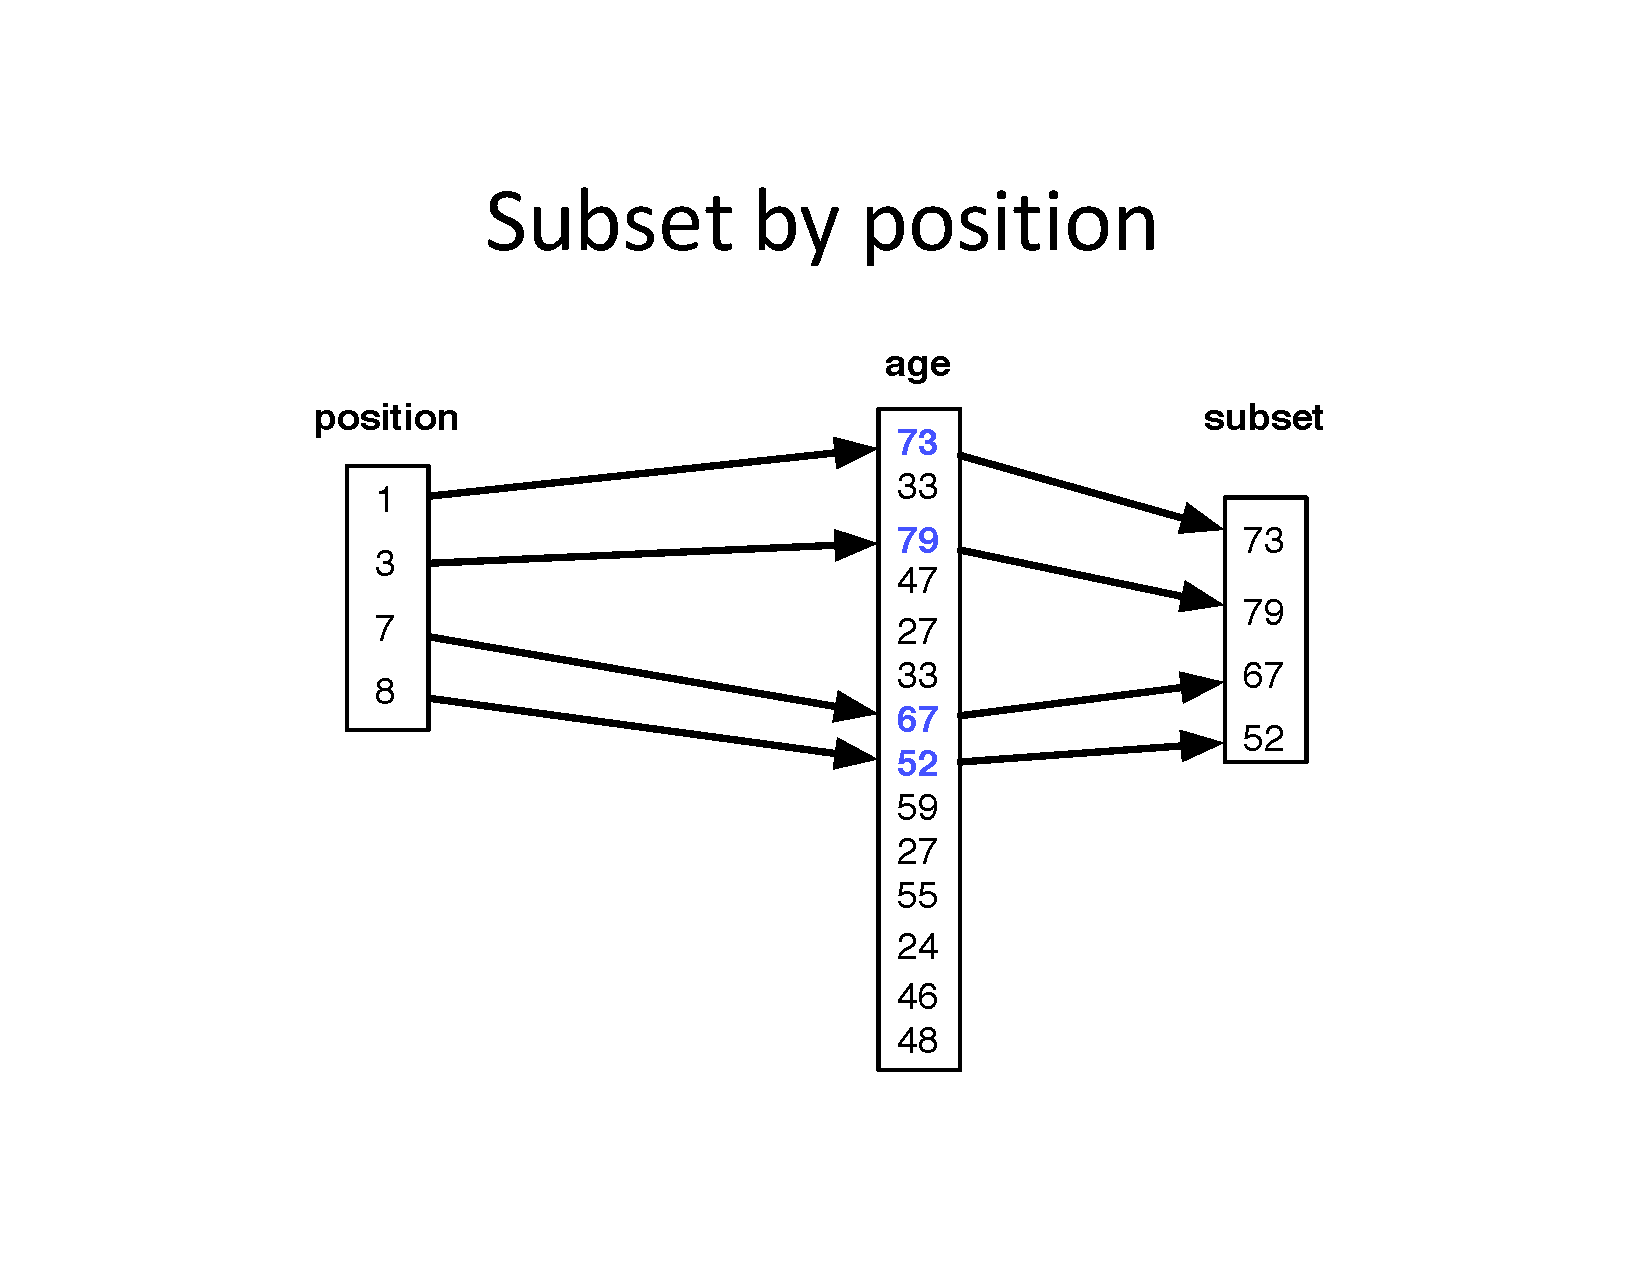
\includegraphics{Subsetpos1.pdf}}}} \par}
  \end{center}
\end{frame}

\begin{frame}[fragile]{Subset by position (2)}
\begin{center}
    {{\resizebox*{1.1\textwidth}{1.1\textheight}
        {\rotatebox{0}{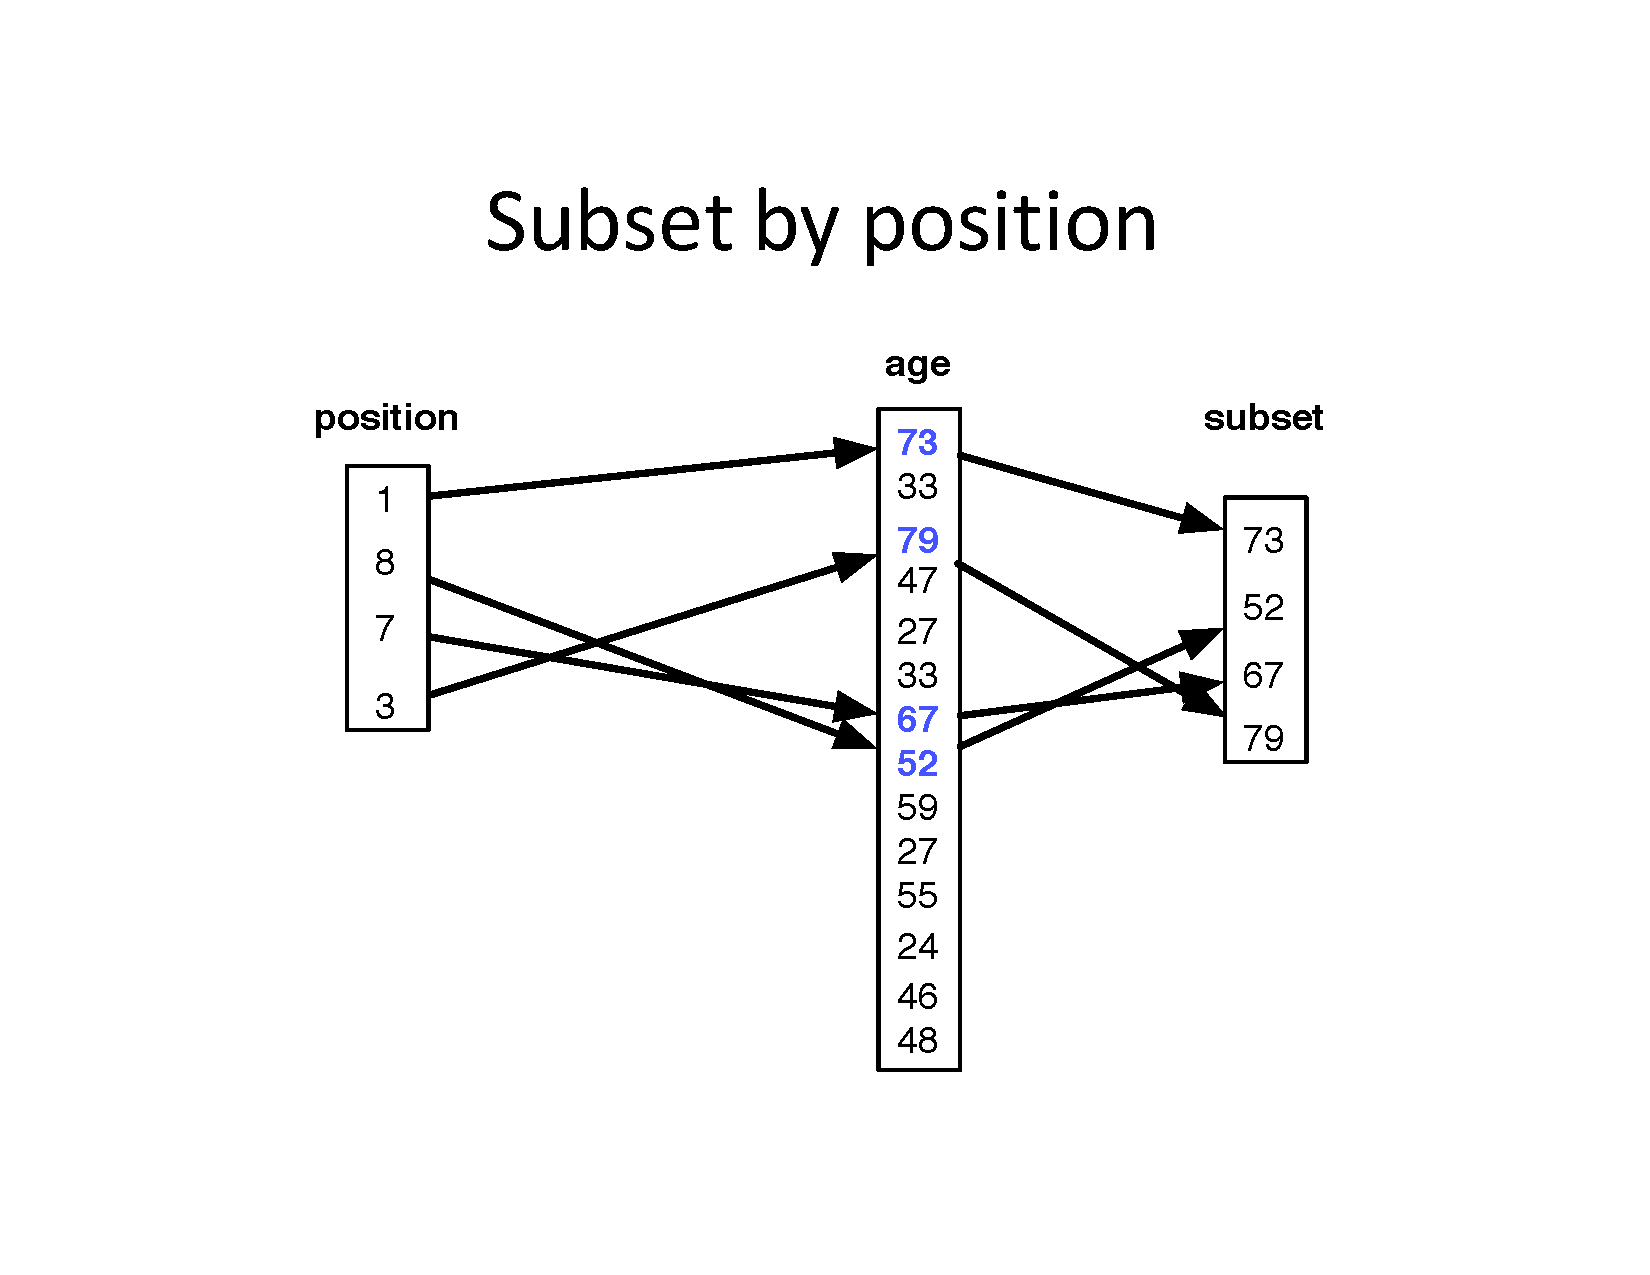
\includegraphics{Subsetpos2.pdf}}}} \par}
  \end{center}

\end{frame}

\begin{frame}[fragile]{Subset by exclusion}
\begin{center}
    {{\resizebox*{1.1\textwidth}{1.1\textheight}
        {\rotatebox{0}{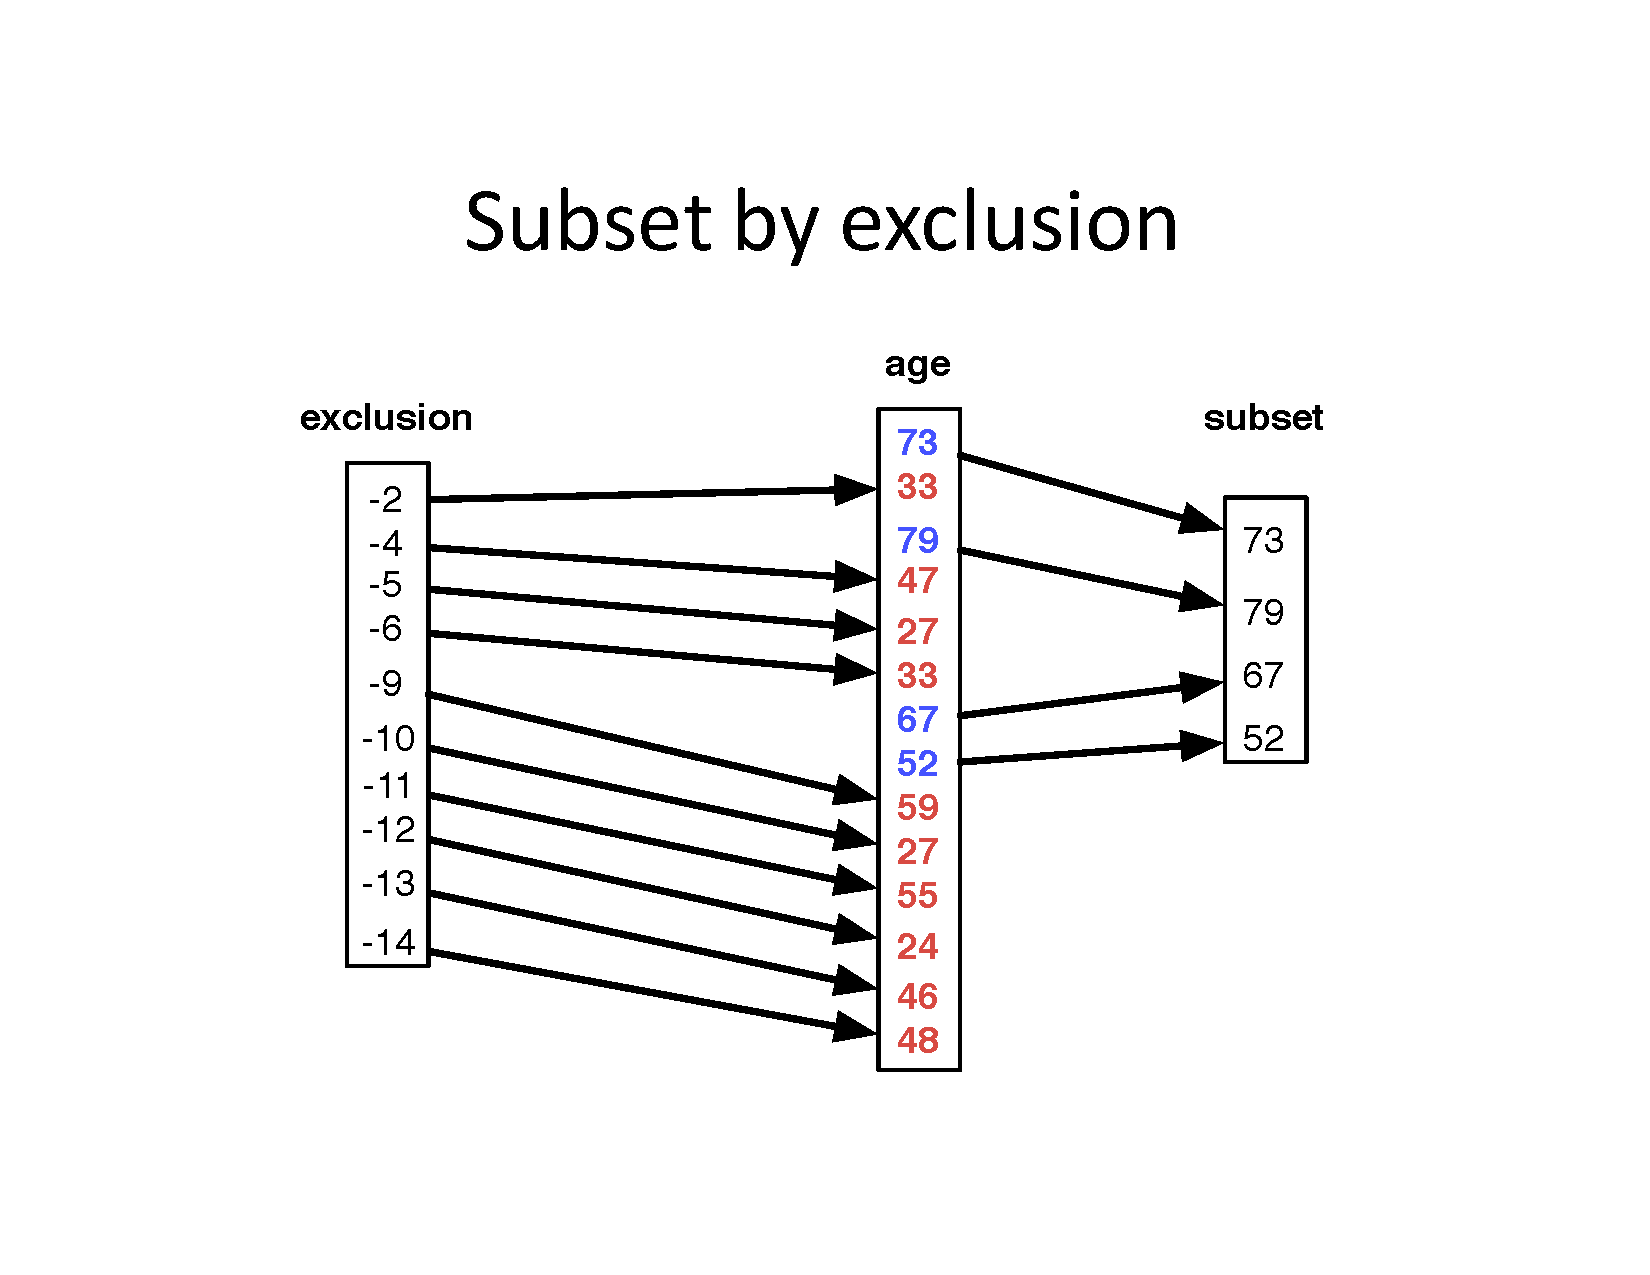
\includegraphics{Subsetexcl.pdf}}}} \par}
  \end{center}
\end{frame}

\begin{frame}[fragile]{Subset by logical}
\begin{center}
    {{\resizebox*{1.1\textwidth}{1.1\textheight}
        {\rotatebox{0}{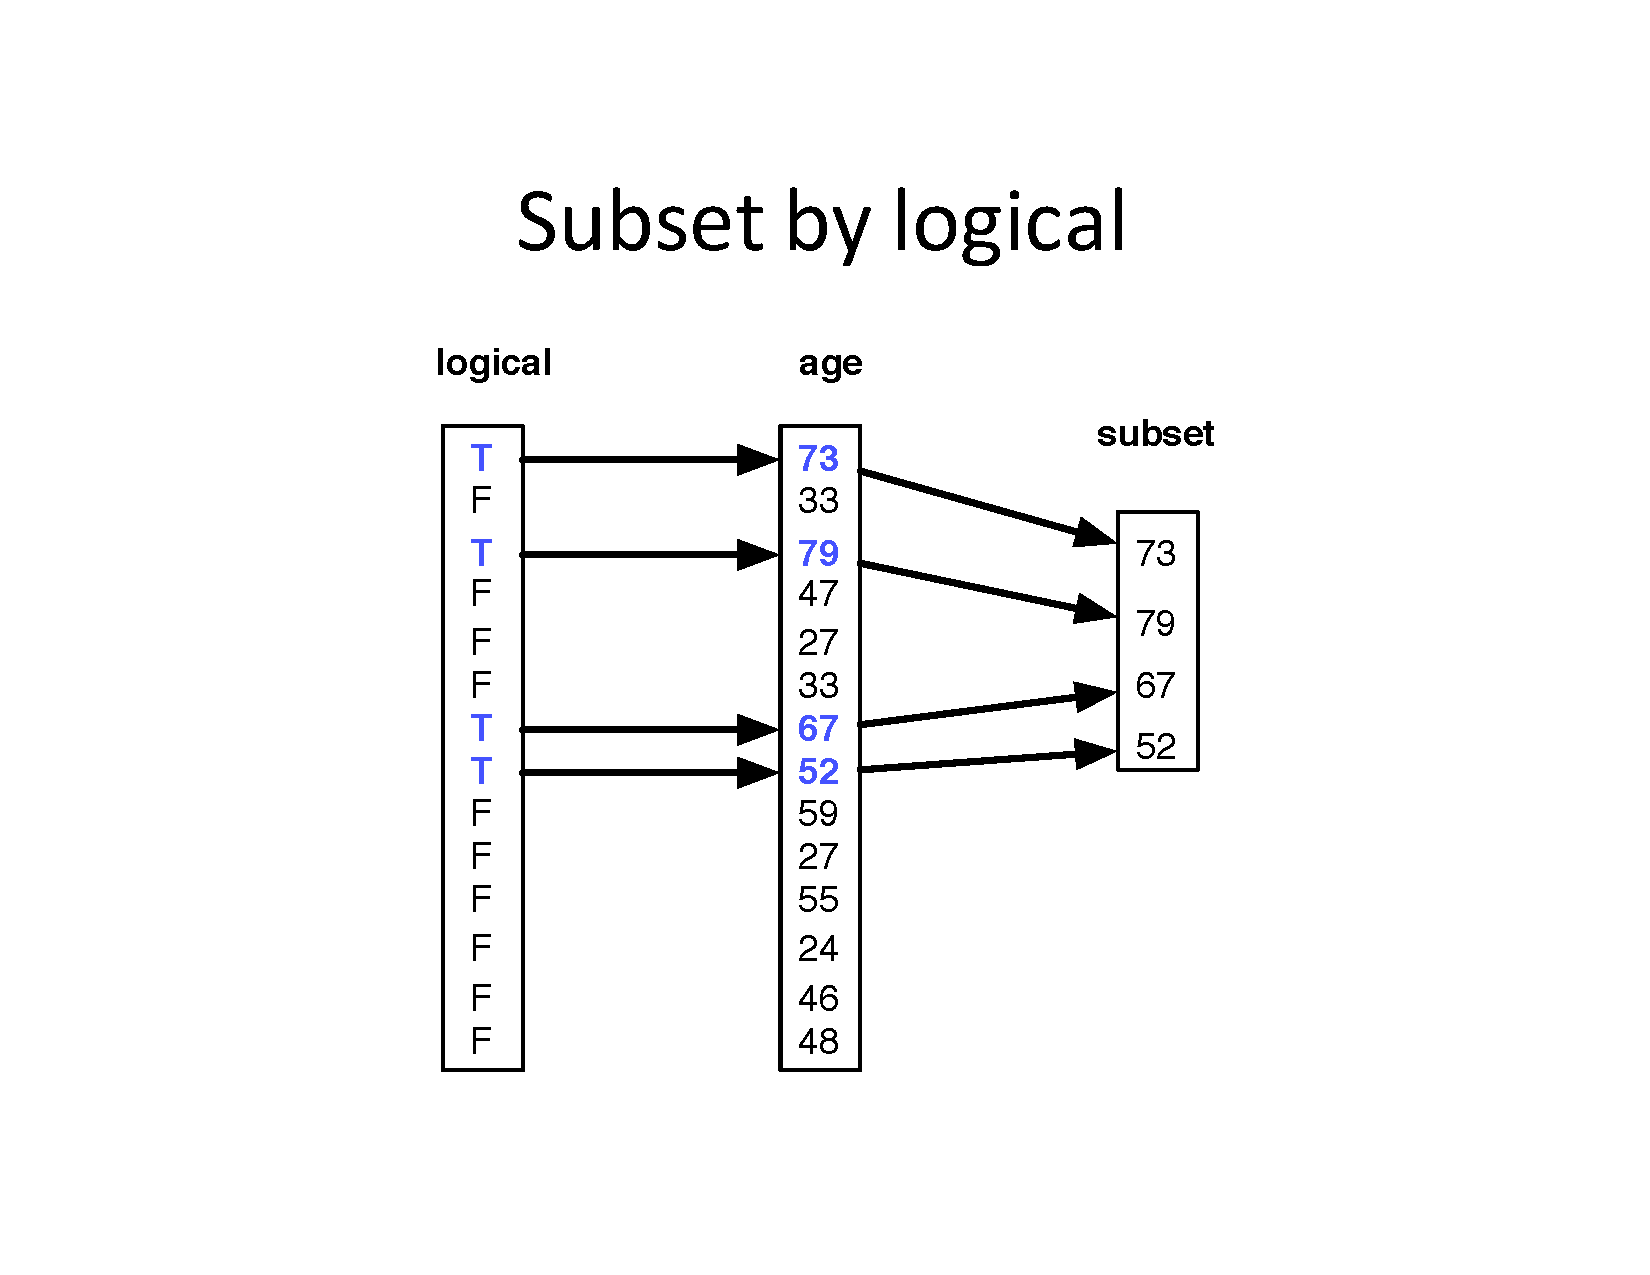
\includegraphics{Subsetlogical.pdf}}}} \par}
  \end{center}
\end{frame}

\begin{frame}[fragile]{Subset by name}
\begin{center}
    {{\resizebox*{1.1\textwidth}{1.1\textheight}
        {\rotatebox{0}{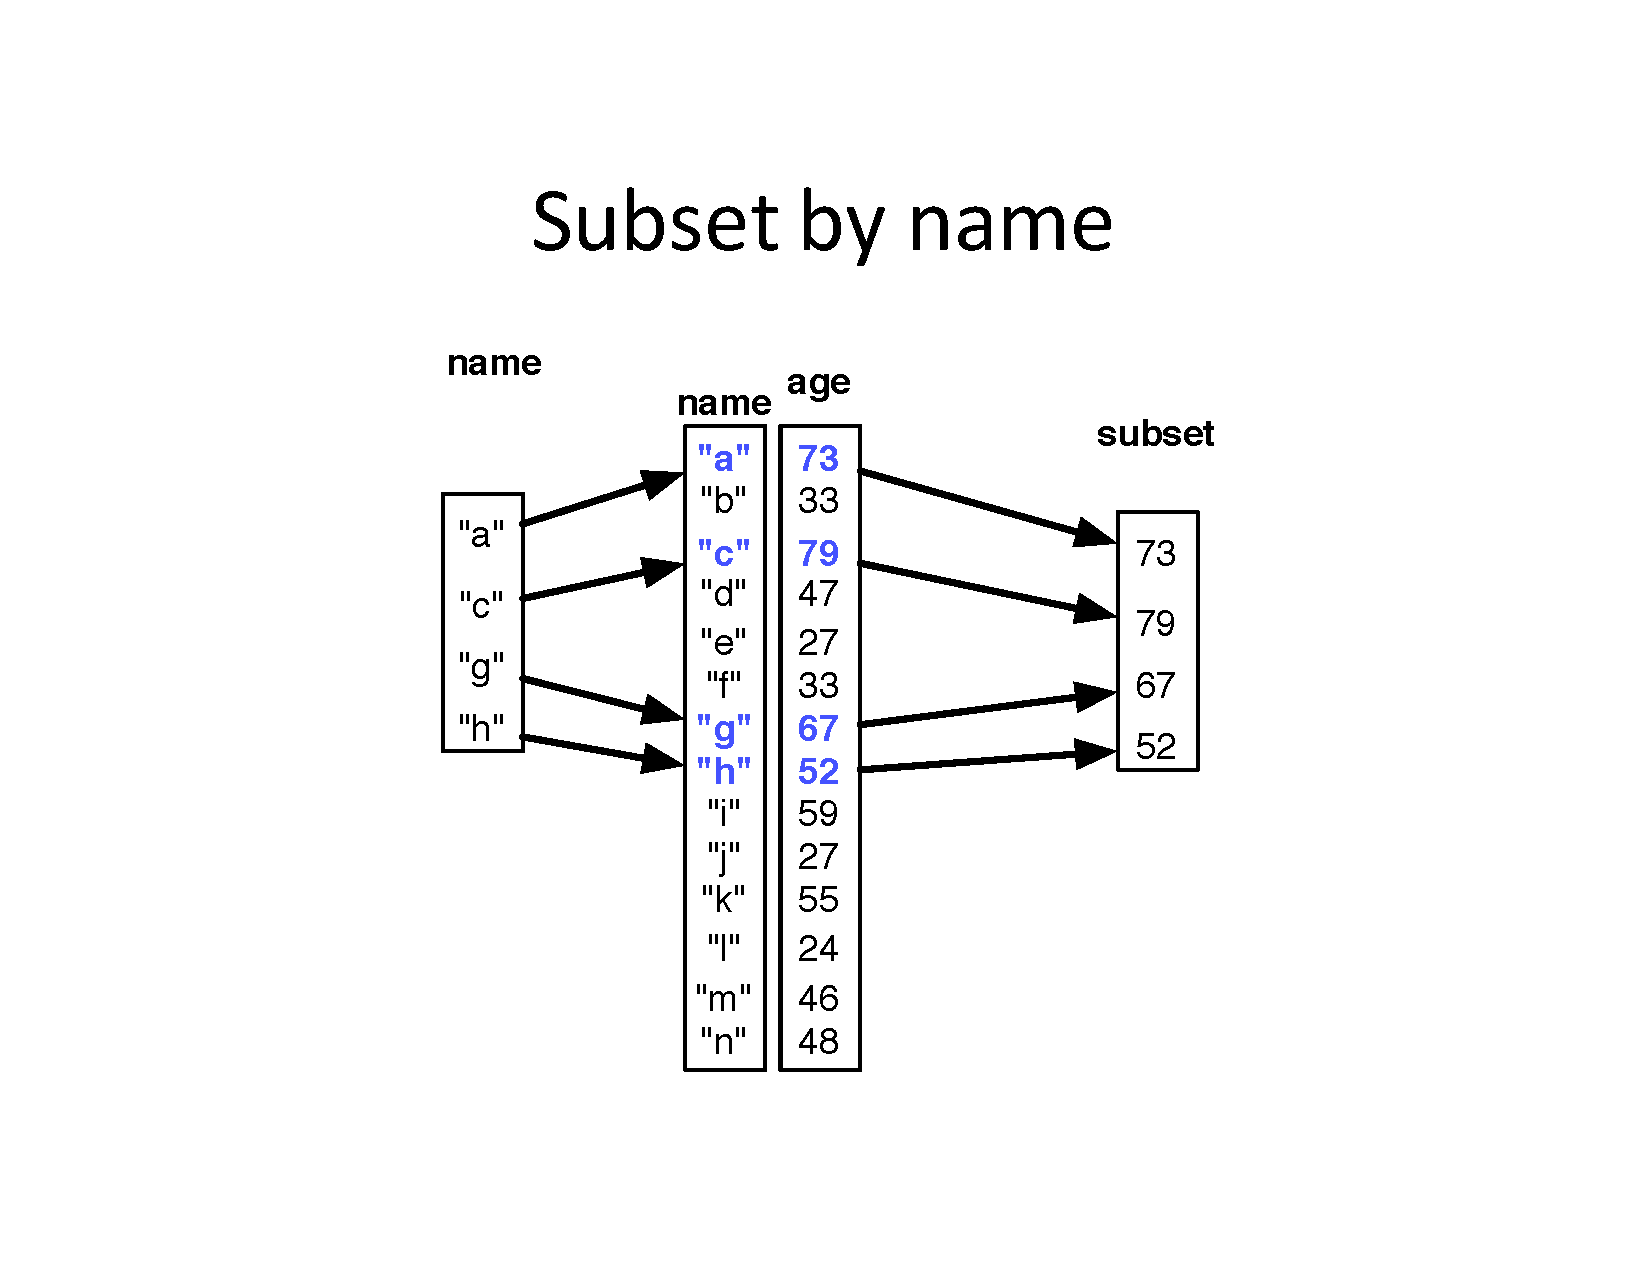
\includegraphics{Subsetname.pdf}}}} \par}
  \end{center}
\end{frame}

\begin{frame}[fragile]{Five ways to subset a vector}
\begin{itemize}
\item Position - indices of the element you want
\item Exclusion - indices of elements to exclude 
\item Logical - logical vector the same length as the vector being subset. Keep the elements corresponding to TRUE. 
\item Name - character vector of names of elements to keep. Vector being subsetted must have names associated with elements
\item All - all the elements
\end{itemize}
\end{frame}

% \begin{frame}[fragile]{Logical operations}
% \begin{itemize}
% \item 
% \end{itemize}
% \end{frame}

\begin{frame}[fragile]{Logical/relational operators}
\begin{itemize}
\item In addition to operators such as +, -, *, and /  R also has logical operators
\item They are relational operators                          $>, <, >=, <=, !=$, and $==$
\item These return a value of TRUE or FALSE
\item They are also vectorized operations
\end{itemize}
\end{frame}

\begin{frame}[fragile]{Examples}
\begin{knitrout}
\definecolor{shadecolor}{rgb}{0.969, 0.969, 0.969}\color{fgcolor}\begin{kframe}
\begin{alltt}
\hlnum{4} \hlopt{<} \hlnum{3}
\end{alltt}
\begin{verbatim}
## [1] FALSE
\end{verbatim}
\begin{alltt}
\hlstr{"a"}\hlopt{==}\hlstr{"A"}
\end{alltt}
\begin{verbatim}
## [1] FALSE
\end{verbatim}
\begin{alltt}
\hlstr{"A"}\hlopt{==}\hlstr{"A"}
\end{alltt}
\begin{verbatim}
## [1] TRUE
\end{verbatim}
\begin{alltt}
\hlnum{4}\hlopt{!=}\hlnum{3}
\end{alltt}
\begin{verbatim}
## [1] TRUE
\end{verbatim}
\end{kframe}
\end{knitrout}
\end{frame}

\begin{frame}[fragile]{}
\begin{knitrout}
\definecolor{shadecolor}{rgb}{0.969, 0.969, 0.969}\color{fgcolor}\begin{kframe}
\begin{alltt}
\hlstd{fweight} \hlopt{>} \hlnum{150}
\end{alltt}
\begin{verbatim}
##  [1]  TRUE FALSE  TRUE  TRUE FALSE  TRUE  TRUE FALSE  TRUE  TRUE  TRUE
## [12] FALSE FALSE FALSE
\end{verbatim}
\begin{alltt}
\hlstd{fsex}\hlopt{!=}\hlstr{"m"}
\end{alltt}
\begin{verbatim}
##  [1] FALSE  TRUE FALSE FALSE  TRUE  TRUE FALSE  TRUE FALSE FALSE  TRUE
## [12] FALSE FALSE  TRUE
\end{verbatim}
\begin{alltt}
\hlstd{fbmi}
\end{alltt}
\begin{verbatim}
##        a        b        c        d        e        f        g        h 
## 25.16239 21.32906 24.45884 24.48414 18.55566 28.94981 28.18797 20.67783 
##        i        j        k        l        m        n 
## 26.66430 30.04911 26.05364 22.64384 24.26126 22.91060
\end{verbatim}
\begin{alltt}
\hlstd{fbmi}\hlopt{==}\hlnum{25.16239}
\end{alltt}
\begin{verbatim}
##     a     b     c     d     e     f     g     h     i     j     k     l 
## FALSE FALSE FALSE FALSE FALSE FALSE FALSE FALSE FALSE FALSE FALSE FALSE 
##     m     n 
## FALSE FALSE
\end{verbatim}
\end{kframe}
\end{knitrout}
% Note: sprintf("%.10f",fbmi[1])
\end{frame}

\begin{frame}[fragile]{Weights of the women in our family}
\begin{itemize}
\item Create a logical expression that identifies the women in the family
\begin{knitrout}
\definecolor{shadecolor}{rgb}{0.969, 0.969, 0.969}\color{fgcolor}\begin{kframe}
\begin{alltt}
\hlstd{fsex}\hlopt{==}\hlstr{"f"}
\end{alltt}
\begin{verbatim}
##  [1] FALSE  TRUE FALSE FALSE  TRUE  TRUE FALSE  TRUE FALSE FALSE  TRUE
## [12] FALSE FALSE  TRUE
\end{verbatim}
\end{kframe}
\end{knitrout}
\item Use this logical expression to subset the vector of fweight
\begin{knitrout}
\definecolor{shadecolor}{rgb}{0.969, 0.969, 0.969}\color{fgcolor}\begin{kframe}
\begin{alltt}
\hlstd{fweight[fsex}\hlopt{==}\hlstr{"f"}\hlstd{]}
\end{alltt}
\begin{verbatim}
## [1] 124  98 190 124 166 125
\end{verbatim}
\end{kframe}
\end{knitrout}
\end{itemize}
\end{frame}

\begin{frame}[fragile]{Boolean algebra}
\begin{itemize}
\item Boolean algebra is a mathematical formalization of the truth or falsity of statements.  
\item It has three operations, “not,” “or,” and “and.”  
\item Boolean algebra tells us how to evaluate the truth or falsity of compound statements that are built using these operations.  For example, if A and B are statements, some compound statements are
\item A and B
\item (not A) or B
\end{itemize}
\end{frame}

\begin{frame}[fragile]{}
\begin{itemize}
\item The "not" operation just causes the statement following it to switch its truth value. \\
So not TRUE is FALSE and not FALSE is TRUE. 
      \item The compound statement A and B is TRUE only if both A and B are TRUE. 
\item The compound statement A or B is TRUE if either or both A or B is TRUE.
\item In R, we write ! for "not," \& for "and," and $|$ for "or."  Note: all of these are vectorized!
\end{itemize}
\end{frame}

\begin{frame}[fragile]{}
\begin{knitrout}
\definecolor{shadecolor}{rgb}{0.969, 0.969, 0.969}\color{fgcolor}\begin{kframe}
\begin{alltt}
\hlopt{!}\hlstd{(fweight} \hlopt{>} \hlnum{150}\hlstd{)}
\end{alltt}
\begin{verbatim}
##  [1] FALSE  TRUE FALSE FALSE  TRUE FALSE FALSE  TRUE FALSE FALSE FALSE
## [12]  TRUE  TRUE  TRUE
\end{verbatim}
\begin{alltt}
\hlstd{(fweight} \hlopt{>} \hlnum{150}\hlstd{)} \hlopt{&} \hlstd{(fnames} \hlopt{==} \hlstr{"Tom"}\hlstd{)}
\end{alltt}
\begin{verbatim}
##  [1]  TRUE FALSE FALSE FALSE FALSE FALSE FALSE FALSE FALSE  TRUE FALSE
## [12] FALSE FALSE FALSE
\end{verbatim}
\begin{alltt}
\hlstd{(fweight} \hlopt{>} \hlnum{150}\hlstd{)} \hlopt{|} \hlstd{(fage} \hlopt{>} \hlnum{65}\hlstd{)}
\end{alltt}
\begin{verbatim}
##  [1]  TRUE FALSE  TRUE  TRUE FALSE  TRUE  TRUE FALSE  TRUE  TRUE  TRUE
## [12] FALSE FALSE FALSE
\end{verbatim}
\end{kframe}
\end{knitrout}
\end{frame}

\begin{frame}[fragile]{Two other functions: all and any}
Guess what these functions are doing:
\begin{knitrout}
\definecolor{shadecolor}{rgb}{0.969, 0.969, 0.969}\color{fgcolor}\begin{kframe}
\begin{alltt}
\hlkwd{all}\hlstd{(fage} \hlopt{>} \hlnum{18}\hlstd{)}
\end{alltt}
\begin{verbatim}
## [1] TRUE
\end{verbatim}
\begin{alltt}
\hlkwd{any}\hlstd{(fage} \hlopt{<} \hlnum{18}\hlstd{)}
\end{alltt}
\begin{verbatim}
## [1] FALSE
\end{verbatim}
\begin{alltt}
\hlkwd{any}\hlstd{(fweight} \hlopt{<} \hlnum{150}\hlstd{)}
\end{alltt}
\begin{verbatim}
## [1] TRUE
\end{verbatim}
\begin{alltt}
\hlkwd{all}\hlstd{(fweight} \hlopt{<} \hlnum{150}\hlstd{)}
\end{alltt}
\begin{verbatim}
## [1] FALSE
\end{verbatim}
\end{kframe}
\end{knitrout}
\end{frame}
\begin{frame}[fragile]{Examples: of all and any}
\begin{knitrout}
\definecolor{shadecolor}{rgb}{0.969, 0.969, 0.969}\color{fgcolor}\begin{kframe}
\begin{alltt}
\hlstd{fage} \hlopt{<} \hlnum{50}
\end{alltt}
\begin{verbatim}
##  [1] FALSE  TRUE FALSE  TRUE  TRUE  TRUE FALSE FALSE FALSE  TRUE FALSE
## [12]  TRUE  TRUE  TRUE
\end{verbatim}
\begin{alltt}
\hlstd{fsex} \hlopt{==} \hlstr{"f"}
\end{alltt}
\begin{verbatim}
##  [1] FALSE  TRUE FALSE FALSE  TRUE  TRUE FALSE  TRUE FALSE FALSE  TRUE
## [12] FALSE FALSE  TRUE
\end{verbatim}
\begin{alltt}
\hlopt{!}\hlstd{foverWt}
\end{alltt}
\begin{verbatim}
##  [1] FALSE  TRUE  TRUE  TRUE  TRUE FALSE FALSE  TRUE FALSE FALSE FALSE
## [12]  TRUE  TRUE  TRUE
\end{verbatim}
\begin{alltt}
\hlstd{(fsex} \hlopt{==} \hlstr{"m"}\hlstd{)} \hlopt{&}\hlstd{(fheight} \hlopt{<} \hlnum{70}\hlstd{)}
\end{alltt}
\begin{verbatim}
##  [1] FALSE FALSE FALSE FALSE FALSE FALSE FALSE FALSE FALSE FALSE FALSE
## [12] FALSE FALSE FALSE
\end{verbatim}
\end{kframe}
\end{knitrout}
\end{frame}

\begin{frame}[fragile]{Examples (contd)}
Previous: Under 50, Women, Not over weight, Males who are under 70 inches tall

\begin{knitrout}
\definecolor{shadecolor}{rgb}{0.969, 0.969, 0.969}\color{fgcolor}\begin{kframe}
\begin{alltt}
\hlstd{fbmi[fnames} \hlopt{==}\hlstr{"Tim"} \hlopt{|} \hlstd{fnames} \hlopt{==} \hlstr{"Tom"} \hlstd{]}
\end{alltt}
\begin{verbatim}
##        a        i        j 
## 25.16239 26.66430 30.04911
\end{verbatim}
\begin{alltt}
\hlstd{fbmi[fheight} \hlopt{>}\hlnum{72}\hlstd{]} \hlkwb{=} \hlnum{NA}
\hlstd{fage[fsex} \hlopt{==} \hlstr{"f"}\hlstd{]} \hlkwb{=}
 \hlstd{fage[fsex} \hlopt{==} \hlstr{"f"}\hlstd{]} \hlopt{+} \hlnum{5}
\end{alltt}
\end{kframe}
\end{knitrout}
Above: BMI of Tim and Tom, Assigns BMI an NA for those over 72 inches tall, Add 5 years to all female ages
\end{frame}

\begin{frame}[fragile]{Use logical expressions to obtain the following subsets}
\begin{knitrout}
\definecolor{shadecolor}{rgb}{0.969, 0.969, 0.969}\color{fgcolor}\begin{kframe}
\begin{alltt}
\hlstd{fage[} \hlopt{!}\hlstd{foverWt ]}
\end{alltt}
\begin{verbatim}
## [1] 38 79 47 32 57 24 46 53
\end{verbatim}
\begin{alltt}
\hlstd{fsex[ fage} \hlopt{>} \hlnum{50} \hlstd{]}
\end{alltt}
\begin{verbatim}
## [1] m m m f m f f
## Levels: f m
\end{verbatim}
\begin{alltt}
\hlstd{fbmi[ fheight} \hlopt{==} \hlkwd{max}\hlstd{(fheight) ]}
\end{alltt}
\begin{verbatim}
##        a        b        c        d        e        f        g        h 
## 25.16239 21.32906 24.45884 24.48414 18.55566 28.94981 28.18797 20.67783 
##        i        j        k        l        m        n 
## 26.66430 30.04911 26.05364 22.64384 24.26126 22.91060
\end{verbatim}
\end{kframe}
\end{knitrout}
Ages of all non-overweight members of the family, Genders of those over 50, BMI of the tallest member of the family
\end{frame}

\begin{frame}[fragile]{Creating vectors}
Concatenate:
\begin{knitrout}
\definecolor{shadecolor}{rgb}{0.969, 0.969, 0.969}\color{fgcolor}\begin{kframe}
\begin{alltt}
\hlkwd{c}\hlstd{(}\hlnum{3}\hlstd{,} \hlnum{2}\hlstd{,} \hlnum{1}\hlstd{)}
\end{alltt}
\begin{verbatim}
## [1] 3 2 1
\end{verbatim}
\begin{alltt}
\hlkwd{c}\hlstd{(}\hlkwc{bob} \hlstd{=}\hlnum{3}\hlstd{,} \hlkwc{alice} \hlstd{=} \hlnum{2}\hlstd{,} \hlkwc{john} \hlstd{=} \hlnum{1}\hlstd{)}
\end{alltt}
\begin{verbatim}
##   bob alice  john 
##     3     2     1
\end{verbatim}
\end{kframe}
\end{knitrout}
\begin{itemize}
\item A vector of three numbers, 3, 2, 1, in that order
\item Elements in a vector – this time with names
\end{itemize}
\end{frame}

\begin{frame}[fragile]{Subset vector based on names}
\begin{knitrout}
\definecolor{shadecolor}{rgb}{0.969, 0.969, 0.969}\color{fgcolor}\begin{kframe}
\begin{alltt}
\hlstd{fheight[}\hlkwd{c}\hlstd{(}\hlstr{"a"}\hlstd{,} \hlstr{"c"}\hlstd{,} \hlstr{"f"}\hlstd{)]}
\end{alltt}
\begin{verbatim}
## [1] NA NA NA
\end{verbatim}
\begin{alltt}
\hlstd{fheight[}\hlkwd{c}\hlstd{(}\hlstr{"a"}\hlstd{,} \hlstr{"f"}\hlstd{,} \hlstr{"f"}\hlstd{,} \hlstr{"c"}\hlstd{)]}
\end{alltt}
\begin{verbatim}
## [1] NA NA NA NA
\end{verbatim}
\end{kframe}
\end{knitrout}
\begin{itemize}
\item Order of names determines order in subset 
\item If we repeat a name we get the element multiple times
\end{itemize}
\end{frame}

\begin{frame}[fragile]{Construct vectors of sequences}
\begin{knitrout}
\definecolor{shadecolor}{rgb}{0.969, 0.969, 0.969}\color{fgcolor}\begin{kframe}
\begin{alltt}
\hlnum{1}\hlopt{:}\hlnum{3}
\end{alltt}
\begin{verbatim}
## [1] 1 2 3
\end{verbatim}
\begin{alltt}
\hlnum{10}\hlopt{:}\hlnum{6}
\end{alltt}
\begin{verbatim}
## [1] 10  9  8  7  6
\end{verbatim}
\begin{alltt}
\hlnum{1.1}\hlopt{:}\hlnum{5.7}
\end{alltt}
\begin{verbatim}
## [1] 1.1 2.1 3.1 4.1 5.1
\end{verbatim}
\begin{alltt}
\hlnum{5.7}\hlopt{:-}\hlnum{1.1}
\end{alltt}
\begin{verbatim}
## [1]  5.7  4.7  3.7  2.7  1.7  0.7 -0.3
\end{verbatim}
\end{kframe}
\end{knitrout}
\begin{itemize}
\item Convenient way to create vectors containing a sequence of numbers
\end{itemize}
\end{frame}

\begin{frame}[fragile]{seq function to construct vectors of sequences}
\begin{knitrout}
\definecolor{shadecolor}{rgb}{0.969, 0.969, 0.969}\color{fgcolor}\begin{kframe}
\begin{alltt}
\hlkwd{seq}\hlstd{(}\hlnum{1}\hlstd{,} \hlnum{6}\hlstd{,} \hlkwc{by} \hlstd{=} \hlnum{2}\hlstd{)}
\end{alltt}
\begin{verbatim}
## [1] 1 3 5
\end{verbatim}
\begin{alltt}
\hlkwd{seq}\hlstd{(}\hlnum{1}\hlstd{,} \hlnum{6}\hlstd{,} \hlkwc{length} \hlstd{=} \hlnum{3}\hlstd{)}
\end{alltt}
\begin{verbatim}
## [1] 1.0 3.5 6.0
\end{verbatim}
\begin{alltt}
\hlkwd{seq}\hlstd{(}\hlkwc{to} \hlstd{=} \hlnum{6}\hlstd{,} \hlkwc{length} \hlstd{=} \hlnum{3}\hlstd{,} \hlkwc{by} \hlstd{=} \hlnum{2}\hlstd{)}
\end{alltt}
\begin{verbatim}
## [1] 2 4 6
\end{verbatim}
\begin{alltt}
\hlkwd{seq}\hlstd{(}\hlkwc{from} \hlstd{=} \hlnum{1}\hlstd{,} \hlkwc{length} \hlstd{=} \hlnum{3}\hlstd{,} \hlkwc{by} \hlstd{=} \hlnum{2}\hlstd{)}
\end{alltt}
\begin{verbatim}
## [1] 1 3 5
\end{verbatim}
\end{kframe}
\end{knitrout}
\begin{itemize}
\item Arguments: from, to, by, length
\end{itemize}
\end{frame}

\begin{frame}[fragile]{Use seq to subset vector}
\begin{knitrout}
\definecolor{shadecolor}{rgb}{0.969, 0.969, 0.969}\color{fgcolor}\begin{kframe}
\begin{alltt}
\hlstd{fbmi[}\hlkwd{seq}\hlstd{(}\hlkwc{from} \hlstd{=} \hlnum{1}\hlstd{,} \hlkwc{to} \hlstd{=} \hlkwd{length}\hlstd{(fbmi),}
       \hlkwc{by} \hlstd{=} \hlnum{2}\hlstd{)]}
\end{alltt}
\begin{verbatim}
##        a        c        e        g        i        k        m 
## 25.16239 24.45884 18.55566 28.18797 26.66430 26.05364 24.26126
\end{verbatim}
\end{kframe}
\end{knitrout}
\end{frame}

\begin{frame}[fragile]{rep command}
\begin{knitrout}
\definecolor{shadecolor}{rgb}{0.969, 0.969, 0.969}\color{fgcolor}\begin{kframe}
\begin{alltt}
\hlkwd{rep}\hlstd{(}\hlnum{3}\hlstd{,}\hlnum{2}\hlstd{)}
\end{alltt}
\begin{verbatim}
## [1] 3 3
\end{verbatim}
\begin{alltt}
\hlstd{x} \hlkwb{=} \hlkwd{c}\hlstd{(}\hlnum{7}\hlstd{,}\hlnum{1}\hlstd{,}\hlnum{3}\hlstd{)}
\hlkwd{rep}\hlstd{(x,} \hlnum{2}\hlstd{)}
\end{alltt}
\begin{verbatim}
## [1] 7 1 3 7 1 3
\end{verbatim}
\begin{alltt}
\hlkwd{rep}\hlstd{(x,} \hlkwd{c}\hlstd{(}\hlnum{3}\hlstd{,} \hlnum{2}\hlstd{,} \hlnum{1}\hlstd{))}
\end{alltt}
\begin{verbatim}
## [1] 7 7 7 1 1 3
\end{verbatim}
\begin{alltt}
\hlkwd{rep}\hlstd{(x,} \hlkwc{each} \hlstd{=} \hlnum{2}\hlstd{)}
\end{alltt}
\begin{verbatim}
## [1] 7 7 1 1 3 3
\end{verbatim}
\end{kframe}
\end{knitrout}
\end{frame}

\begin{frame}[fragile]{Repeat characters}%{Vector of last names}
\begin{knitrout}
\definecolor{shadecolor}{rgb}{0.969, 0.969, 0.969}\color{fgcolor}\begin{kframe}
\begin{alltt}
\hlstd{flastnames} \hlkwb{=} \hlkwd{rep}\hlstd{(}\hlstr{"Smith"}\hlstd{,}\hlkwc{times} \hlstd{=} \hlkwd{length}\hlstd{(fbmi))}
\hlstd{flastnames} \hlkwb{=} \hlkwd{character}\hlstd{(}\hlkwc{length} \hlstd{=} \hlkwd{length}\hlstd{(fbmi))}
\hlstd{flastnames[ ]} \hlkwb{=} \hlstr{"Smith"}
\end{alltt}
\end{kframe}
\end{knitrout}
\begin{itemize}
\item vector where repeat "Smith" multiple (length of fbmi) times
\item vector of characters multiple (length of fbmi) times
\item each element of this vector gets "Smith"
\end{itemize}
\end{frame}

\begin{frame}[fragile]{Producing vectors without typing all values out}%{Vector of last names}
\begin{knitrout}
\definecolor{shadecolor}{rgb}{0.969, 0.969, 0.969}\color{fgcolor}\begin{kframe}
\begin{alltt}
\hlkwd{rep}\hlstd{(}\hlkwd{seq}\hlstd{(}\hlnum{0}\hlstd{,} \hlnum{8}\hlstd{,} \hlkwc{by} \hlstd{=} \hlnum{2}\hlstd{),} \hlkwc{each} \hlstd{=} \hlnum{5}\hlstd{)}
\end{alltt}
\begin{verbatim}
##  [1] 0 0 0 0 0 2 2 2 2 2 4 4 4 4 4 6 6 6 6 6 8 8 8 8 8
\end{verbatim}
\begin{alltt}
\hlkwd{rep}\hlstd{(}\hlnum{1}\hlopt{:}\hlnum{5}\hlstd{,} \hlnum{5}\hlstd{)}
\end{alltt}
\begin{verbatim}
##  [1] 1 2 3 4 5 1 2 3 4 5 1 2 3 4 5 1 2 3 4 5 1 2 3 4 5
\end{verbatim}
\begin{alltt}
\hlkwd{rep}\hlstd{(}\hlnum{1}\hlopt{:}\hlnum{5}\hlstd{,} \hlnum{5}\hlstd{)} \hlopt{+} \hlkwd{rep}\hlstd{(}\hlnum{0}\hlopt{:}\hlnum{4}\hlstd{,} \hlkwc{each} \hlstd{=} \hlnum{5}\hlstd{)}
\end{alltt}
\begin{verbatim}
##  [1] 1 2 3 4 5 2 3 4 5 6 3 4 5 6 7 4 5 6 7 8 5 6 7 8 9
\end{verbatim}
\end{kframe}
\end{knitrout}
\begin{itemize}
\item Code to produce 
0 0 0 0 0 2 2 2 2 2 4 4 4 4 4 6 6 6 6 6 8 8 8 8 8?
\end{itemize}
\end{frame}

\begin{frame}[fragile]{sort function}%{Vector of last names}
\begin{knitrout}
\definecolor{shadecolor}{rgb}{0.969, 0.969, 0.969}\color{fgcolor}\begin{kframe}
\begin{alltt}
\hlstd{fage}
\end{alltt}
\begin{verbatim}
##  [1] 77 38 79 47 32 38 67 57 59 27 60 24 46 53
\end{verbatim}
\begin{alltt}
\hlkwd{sort}\hlstd{(fage)}
\end{alltt}
\begin{verbatim}
##  [1] 24 27 32 38 38 46 47 53 57 59 60 67 77 79
\end{verbatim}
\begin{alltt}
\hlkwd{sort}\hlstd{(fage,} \hlkwc{decreasing} \hlstd{=} \hlnum{TRUE}\hlstd{)}
\end{alltt}
\begin{verbatim}
##  [1] 79 77 67 60 59 57 53 47 46 38 38 32 27 24
\end{verbatim}
\end{kframe}
\end{knitrout}
\end{frame}

\begin{frame}[fragile]{order function}%{Vector of last names}
\begin{knitrout}
\definecolor{shadecolor}{rgb}{0.969, 0.969, 0.969}\color{fgcolor}\begin{kframe}
\begin{alltt}
\hlstd{fage}
\end{alltt}
\begin{verbatim}
##  [1] 77 38 79 47 32 38 67 57 59 27 60 24 46 53
\end{verbatim}
\begin{alltt}
\hlkwd{order}\hlstd{(fage)}
\end{alltt}
\begin{verbatim}
##  [1] 12 10  5  2  6 13  4 14  8  9 11  7  1  3
\end{verbatim}
\end{kframe}
\end{knitrout}
order tells us 12th element of fage is smallest, the 5th is the second smallest,...
This function has a decreasing argument too. 
\end{frame}

\begin{frame}[fragile]{Assign values to elements of a vector}
\begin{knitrout}
\definecolor{shadecolor}{rgb}{0.969, 0.969, 0.969}\color{fgcolor}\begin{kframe}
\begin{alltt}
\hlstd{fheight}
\end{alltt}
\begin{verbatim}
## [1] 70
\end{verbatim}
\begin{alltt}
\hlstd{fheight[}\hlnum{2}\hlstd{]} \hlkwb{=} \hlnum{61}
\hlstd{fheight[}\hlopt{-}\hlnum{13}\hlstd{]} \hlkwb{=} \hlnum{62}
\hlstd{fheight[}\hlstr{"e"}\hlstd{]} \hlkwb{=} \hlnum{67}
\hlstd{fheight[overWt]} \hlkwb{=} \hlnum{NA}
\end{alltt}


{\ttfamily\noindent\bfseries\color{errorcolor}{\#\# Error in fheight[overWt] = NA: object 'overWt' not found}}\begin{alltt}
\hlstd{fheight[]} \hlkwb{=} \hlnum{70}
\hlstd{fheight} \hlkwb{=} \hlnum{70}
\end{alltt}
\end{kframe}
\end{knitrout}
By inclusion, exclusion, name, logical, all
\end{frame}

\begin{frame}[fragile]{}
\begin{knitrout}
\definecolor{shadecolor}{rgb}{0.969, 0.969, 0.969}\color{fgcolor}\begin{kframe}
\begin{alltt}
\hlstd{fheight[foverWt]}
\end{alltt}
\begin{verbatim}
## [1] 70 NA NA NA NA NA
\end{verbatim}
\begin{alltt}
\hlstd{fheight}
\end{alltt}
\begin{verbatim}
## [1] 70
\end{verbatim}
\begin{alltt}
\hlstd{fheight[]} \hlkwb{=} \hlnum{70}
\hlstd{fheight}
\end{alltt}
\begin{verbatim}
## [1] 70
\end{verbatim}
\begin{alltt}
\hlstd{fheight} \hlkwb{=} \hlnum{70}
\end{alltt}
\end{kframe}
\end{knitrout}
By inclusion, exclusion, name, logical, all
\end{frame}

\begin{frame}[fragile]{Summary of functions}
\begin{itemize}
\item c()
\item :
\item seq()
\item rep()
\item sort()
\item order()
\end{itemize}
\end{frame}

\end{document}



